\documentclass[12pt,oneside]{fithesis2}
\usepackage[english]{babel}
\usepackage[utf8]{inputenc}
\usepackage[T1]{fontenc}
\usepackage{fixltx2e}
\usepackage[plainpages=false,pdfpagelabels,unicode]{hyperref}
\usepackage{indentfirst}
\usepackage{setspace}
\usepackage{listings}
\usepackage{graphicx}
\usepackage{float}
\usepackage{mathtools}
\thesistitle{Real-time collaboration in Komodo} 
\thesislogo{fi-logo.mf}
\thesissubtitle{Master's thesis}
\thesisstudent{Bc. Matúš Makový} 
\thesiswoman{false} 
\thesislang{en} 
\thesisfaculty{fi}
\thesisyear{Spring 2015}
\thesisadvisor{RNDr. Filip Nguyen} 
\setstretch{1.2}
\begin{document}
\FrontMatter
\ThesisTitlePage
\begin{ThesisDeclaration}
\DeclarationText
\AdvisorName
\end{ThesisDeclaration}
\begin{ThesisThanks}
%Thank you
\end{ThesisThanks}
\begin{ThesisAbstract}
%Abstract
\end{ThesisAbstract}
\begin{ThesisKeyWords}
%Keywords
\end{ThesisKeyWords}
\tableofcontents 
\MainMatter
\chapter{Introduction} 
Many software solutions enable people to create new things in a better and faster way. In most cases the resulting product should be so complex that one person is not enuogh for the successful and fast creation. Creators try to collaborate to achive a common goal. Among other opportunities and possibilities are collaboration and sharing the greatest benefits of the Internet. \par
At the beginning, as the Internet didn't have such capacity, people tried to use it just for sharing their drafts of work and sending them to each other. This enabled creators to copperate, but they could not work at the same time without having to synchronize their drafts. In other words, they had to find differences between their drafts and reflect them to each other's version. Information technologies had solution for this called Revision control. It had also many limitations, for example 2 people could not edit the same file in a project without having to resolve confilicts manualy when they tried to merge their work with collaborator's version\par
With the development of the Internet came a reasonable solution called real-time collaboration. Using this principle, author can see what his collaborator is doing in real-time and the manual synchronization or manual confilict resolution is not necessary. Information technologies take care of this synchronization and conflict resolution for the users.\par
In the theoretical part of this thesis, author deals with principles of real-time collaboration and describes some of the techniques used to implement real-time collaboration in software over the Internet. There is also a comparison of these techniques from various aspects. The practical part of this thesis deals with JBoss Data Virtualization and Komodo software as a new version of Teiid Designer developed by Red Hat that should use real-time collaboration in its upcomming release. Author recommends best technique for this authoring software regarding the requirements of data models and finds a suitable implementation in Java programming language.

\chapter{Real-time collaboration}
This chapter covers the basic overview of collaboration in general, description of real-time collaboration and description of difficulties with its implementation over the Internet. Last sections of this chapter describe three techniques used for implementation over the Internet and its properties. Techniques described in this chapter are: Operational Transformation, Differential Synchronization and Commutative replicated data types.
\section{Basic overview}
Collaboration, as defined by English dictionary, is an act of working with another or others on a joint project.[cit] Systems that support collaboration are called Groupware. \par Groupware systems are computer-based systems that support \\two or more users engaged in a common task, and that provide an interface to a shared environment. These systems frequently require fine-granularity sharing of data and fast response times.\cite{Ellis} We can identify 2 types of collaboration over the Internet, non real-time collaboration and real-time collaboration.\par
In non real-time collaboration users work on separate copies of a project and then need to merge their changes into one final project. This type of collaboration needs to have a common shared repository in which both users commit their changes. It doesn't offer such flexibility as real-time collaboraion. Users have to check with each other on what part of project are they working, because the confilict resolution in such systems is not ideal and confilict has to be resolved manually. Examples of non real-time collaboration could be Revision control (Git, SVN), (TO DO) . \par When using real-time collaboration, software creates an illusion that users are working on one shared copy of a document online. There is no requirement to commit changes to some kind of repository. Changes are reflected and saved immediately. Examples of real-time collaborative editors are Google Docs, Etherpad and Google Wave. \par Software engineer has different options for implementetation of real-time collaboration in software solution. \par Requirements for a good technique are: 
\begin{itemize}
\item speed
\item latency tolerantion
\item low data transfer
\item consistency maintanance
\item good conflict resolution
\end{itemize}
\par The speed requirement means that changes made on one side of the collaboration process need to be reflected to the other sides as soon as possible and vice versa. Changes should be sent to other collaborators as soon as they are done. If a collaboration technique is fast enough it is much easier to satisfy other requirements on this technique. Fast enough technique is able to maintain good consistency. The system’s response time is the time necessary for the actions of one user to be reflected by their own interface; the notification time is the time necessary for one user’s actions to be propagated to the remaining users’ interfaces.\cite{Ellis} Response time and notification time should be as short as possible.  \par One of the problems of real-time collabarative editing could be the latency of the network, here comes the latency toleration requirement. Implemented technique should be able to tollarate the latency of internet connections, because collaborators could be in very distinct parts of the world. It should be able to reconstruct the right order of operations because packets sent over the Internet don't necessary come in right order and the order of the operations is ery important to maintain consistency.\par Low data transfer requirement is also very important. Different sides of the collaboration should send as few data as possible. Transfered data should only describe change that has been done on one side of collaboration, it is not necessary to transfer the whole project. The less data is needed to transfer the faster the whole protocol can be.  \par Consistency maintanance is necesssary for the success, it has to be ensured, that users on both sides are looking and the same version of a document regardless of number and coplexity of operations done on both sides of the collaboration. Lack of consistency could cause other problems and chaos in the document versions. According to \cite{Vidot} there are three problems encountered when trying to achive consistency maintenance and they correspond to the properties of CCI consistency model proposed in \cite{Sun}
\begin{enumerate}
\item \textbf{Casuality Preservation} - operation \(O_{1}\) causually precedes operation \(O_{2}\) if \(O_{1}\) occured localy before \(O_{2}\). The problem is to execute operations in right order on all sites.
\item \textbf{User Intension Preservation} - technique must preserve user's intension in the context of state, in which the operation was executed. This problem is in strog relation with confilict resolution requirement and occures when we can not determine if \(O_{x}\) casually precedes \(O_{y}\) or \(O_{y}\) casually precedes \(O_{x}\).
\item \textbf{Convergence} - when same operations have been applied on every site, the documents are identical.
\end{enumerate}
\par Because the real-time collaboration is asychnronious there rises a problem of concurency. This means, that changes can happen at the same time and in the same sections of project. Good conflict resolution requirement is present because of concurency. Implementation techniques have to be able to identify and resolve a conflict when users are editing the same part of the project. \par The concurrency control algorithms are separeted in two classes: pessimistic and optimistic. \par Pessimistic algorithms require communication with other sites or with a central coordinator before making a change to data. \par Optimistic concurrency control, on the other hand, requires no communication before applying changes locally. The party making a change applies it immediately, then informs the other parties of the action. If more than one participant makes a change at the same time, a conflict resolution algorithm creates compensating changes to move everyone to the same final state.\cite{Jupiter} This implies that optimistic algorithms are better solution for Internet, because we can not guarantee the latency.
\section{Operational Transformation}
\par Operational transformation (OT) is optimistic concurrency control algorithm used for real-time collaborative editing over the Internet. 
\par It was first introduced in paper Concurency Control in Groupware Systems\cite{Ellis} in 1989, together with The Distrubeted Optional Transformation (dOPT) Algorithm. As the paper describes it, algorithm has a number of properties which make it suitable for groupware. First, operations are performed immediately on their originating site, thus responsiveness is good. Secondly, locks are not necessary so all data remains accessible to group members. Finally, the algorithm is fully distributed, and resilient to site failure. \par This first algorithm was able to process only plain text. Later some problems with correctnes were discovered and resolved in following works. Over the years many other algorithms implementing OT have been published. Algorithms used today are able to process also XML and other formats. \par OT was used also in Jupiter Collaboration System in 1995 \cite{Jupiter}. Jupiter's two-way algorithm is derived from the dOPT algorithm used by Grove in \cite{Ellis}. This algrithm is one of the imporovments of dOPT. \par Today is Google one of the most common implementators of this protocol. The main application was in Google Wave project, which is now terminated , although Operational Transformation found application also in Google Docs project. According to \cite{Spiewak} Google is one of the bigest inovators of this approach an it's biggest contribution is the idea of operation compositon, which is described later in this section. \par The approches differ also in the architecture, dOPT doesn't involve server in its design, but the recent algorithms use a central server.
\par This section will explain basic principles of Operational transformation using Google version of the algorithm and then introduce other algorithms, like dOTP, Jupiter and AT(TIPS). It will also point out the differences in this algorithms compared to Google OT. 
\par The basic idea is that data are replicated on every machine and the only information that is sent over the Internet are the operations. Data replication ensures good responsivnes in high latency enviroments. Wave's addition to OT are also annotations. An annotation is some meta-data associated with an item range, i.e., a start position and an end position. This is particularly useful for describing text formatting and spelling suggestions, as it does not unecessarily complicate the underlying structured document format.\cite{Google} \par The main building block of this approach, as the name suggests, is an operation. Here are some operations defined for use in Google Wave\cite{Google}:
\begin{itemize}
\item retain() - move cursor
\item insertCharacters() - inserts texts
\item insertElementStart() - inserts starting tag
\item insertElementEnd() - inserts end tag
\item deleteCharacters() - deletes text
\item deleteElementStart() - deletes starting tag
\item deleteElementEnd() - deletes ending tag
\item replaceAttributes() - replaces attributes in tag
\item updateAttributes() - updates attributes in tah
\item annotationBoundary() - describes changes in annotations
\end{itemize}
\par The operation is executed locally and then sent over the network to the server or to other peers, to execute the operation on their version of the document. Every object that can be changed in the document has its index for identification. Google Wave uses XML as format for storing information so as an object is considered a character in text and also a starting and terminating tag in XML structure (characters of tags are not considered elements). 
\par The second major part of this technique is a transformation function, that transforms operations. Operations which are sent over the network and recieved by server can not be executed directly on the server's version of the document, because the index of the desired element could be different in the local copy and in the server copy of the document and this can cause inconsistency and violation of User Intension Preservation. 
\par See Figure 2.1 with example for better explanation. For the purpose of this example, let's assume we have one peer that sends operations done on his local copy and a server that recieves operations from all peers and maintains server version of the document. 
\begin{figure}[H]
\caption{Example Operational Transformation}
\centering
\vspace{5mm}
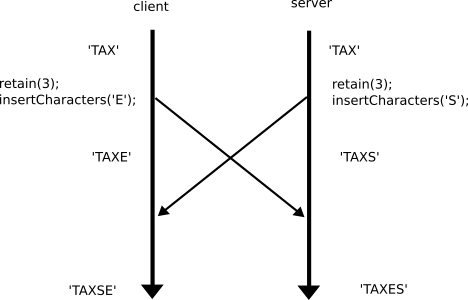
\includegraphics{example}
\end{figure}
Both of them start with text 'VWXYZ' in their document. Peer wants to delete character 'X' so he executes operations:
\vspace{3mm}
\begin{verbatim}
retain(3);
deleteCharacters(1);
\end{verbatim} 
\vspace{3mm}
In the meantime server recieved operation from other peer, that wants to delete character 'Y' and this peer has won in race condition on server, so server executes operations:
\vspace{3mm} 
\begin{verbatim}
retain(4);
deleteCharacter(1);
\end{verbatim}
\vspace{3mm}
Different order and change of indexes on both sides of the collaboration result in incosistent document state. String in first document is 'VWY' and string in second document is 'VWZ'.  In order to preserve user's intension and to reach correct result we have to transform this operations. The correct result after deleting letters 'X' and 'Y' should be 'VWZ'. The server has correct result but the peer doesn't so we have to transform the operation sent by server to look like this:
\vspace{3mm}
\begin{verbatim}
retain(3);
deleteCharacter(1);
\end{verbatim}
\vspace{3mm}
After this change the result of applying operations on both sides will be correct.\par More gernerally, if we have two operations \(O_{1}\) and  \(O_{2}\) we need a transformation function \textit{trasform}, such that: 
\begin{center}
\(transform(O_{1},O_{2}) = (O'_{1},O'_{2}) \land O_{1} \circ O'_{2} \equiv O_{2} \circ O'_{1} \) 
\end{center}
In other words, the function takes two operations and transforms them against each other and the output of the function are two transformed operations, such that, if we have same strings on both sides a we apply \( O_{1} \) and \(O'_{2}\) on one side, and \( O_{2} \) and  \( O'_{1} \) on the other side, the resulting string is the same. This problem could be also described as a "diamond problem". See Figure 2.2.
\begin{figure}[H]
\caption{Diamond problem - 1}
\centering
\vspace{5mm}
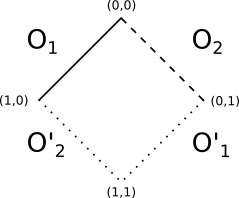
\includegraphics{diamond}
\end{figure}
Operations done by peer take the document to the left side and operations done on server take the document to the right side. Each node in the diamond diagram is representation of the number of operations done by peer and server in particular state. \par As for the example, the correct scenario would be that peer and server exchange their operations, each one computes its transformation and applies the transformated operation on their versions of documents.\par The problem presented by this example is acctually the only one that is Operational Transformation capable of solving. Complicated sittuation occurs when the amount of operations done by one side of the collaboration is greater then on the other side. 
\begin{figure}[H]
\caption{Diamond problem - 2}
\centering
\vspace{5mm}
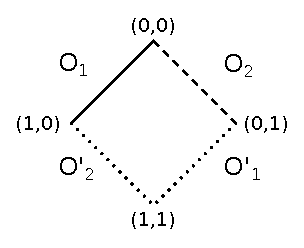
\includegraphics{diamond1}
\end{figure}
On the server side, the server computes tranformation for operations (a,c), applies operation a' on its version of the document. The remaining operation c' has to be preserved for the next transformation. In the next step server must use b and c' as an input and computes b' that can be applied on its version of the document. Server's document is in the desired state. \par On the client side, peer has to transform c against two operations to get to desired state. For two operations it is not a big problem, but as the number of operations could very quickly increase, because client doesn't have to wait for the server to accept and acknowledge his operations, it could be potecially take long time. One of the advantages of Google Wave Operational Transformation is that it is able to compose the operations if they are compatible. This Composer is able to validate operations to make sure that they are compatible and compose them. If operations a and b are composed into operation d, tranformation function can take operations (d,c) and produce operation c'' that can be applied to peer's document and the document is in desired state.   
\section{Differential Synchronization}
\section{Commutative Replicated Data Types}
\chapter{Comparison of Techniques}
\section{Comparison Criteria}
\section{Comparison}
\chapter{Komodo}
\section{Overview}
\section{Komodo Requirements for Real-time Collaboration}
\section{Best Technique for Komodo}
\section{Java Implementation}
\chapter{Conclusion}
\bibliographystyle{acm} 
\bibliography{bib-db} 
\end{document}
